\chapter{Introducción y objetivos}\label{cap.introduccion}
El objetivo general de este trabajo se sitúa en  entender el funcionamiento del aprendizaje profundo con redes neuronales, utilizando para ello una de las plataformas existentes para el desarrollo de las mismas, Caffe.\\

En este capítulo se situará el trabajo en el marco existente en la actualidad, explicando de manera genérica en qué consiste el aprendizaje profundo, el por qué del uso de una determinada plataforma y los problemas que es posible abordar con esta técnica. Además, se expondrán los objetivos concretos de este proyecto, la metodología empleada para alcanzarlos y un pequeño resumen de cómo se ha estructurado el trabajo.

\section{Contexto y motivación}

Desde que los primeros ordenadores fueron programados, el ser humano se ha planteado la posibilidad de conseguir que estas máquinas adquieran inteligencia, logrando que realicen tareas propias de las personas permitiendo, por ejemplo, automatizar el trabajo de rutina, entender el habla o las imágenes, hacer diagnósticos en medicina y apoyar la investigación científica básica. Hoy en día, la \acrfull{ia}~\cite{Goodfellow-et-al-2016}, como se determina al campo que desarrolla estas tareas, cada vez adquiere más presencia, con un alto potencial por sus muchas aplicaciones prácticas y temas de investigación activos.\\

En el nacimiento de la \acrshort{ia} se abordaron y resolvieron rápidamente problemas que son intelectualmente difíciles para los seres humanos, pero relativamente sencillos para los ordenadores, problemas que pueden describirse mediante una lista de reglas formales y matemáticas. Una meta actual aún más ambiciosa consiste en resolver las tareas que son fáciles de realizar para las personas, pero difíciles de describir formalmente, esos problemas que son resueltos de manera rápida e intuitiva por el ser humano como, por ejemplo, el reconocimiento visual de las personas.\\

La {ia} abarca varios campos y en este trabajo el foco estará puesto sobre la \acrfull{va}. La \acrshort{va} trata de analizar y procesar las imágenes del mundo real de tal manera que un ordenador pueda establecer conclusiones sobre las mismas. La idea básica es tratar de trasladar a una máquina la forma en que el ser usa sus ojos y su cerebro para comprender el mundo que le rodea, permitiendo a las mismas tomar decisiones y actuar según la situación. Para conseguir esta comprensión de las máquinas es necesario aplicar conocimientos de distintos campos como la geometría, la estadística, la física y otras disciplinas.\\

Para conseguir materializar el concepto de la \acrshort{va} se hace uso de las \acrfull{rna}. Estas redes están compuestas por capas de neuronas interconectadas que tratan de imitar el comportamiento de las mismas en el cerebro del ser humano. La neurona biológica, consta de un cuerpo celular (soma) del que surge un denso árbol de ramificaciones (dendritas) y una fibra tubular (axón). Esta estructura se asemeja a un procesador de información simple formado por un canal de entrada, similar a las dentritas, un procesador, cuya función se asemeja a la del soma, y un canal de salida, equiparable al axón. Además, entre las neuronas biológicas se establecen una serie de conexiones unidireccionales, conocidas como sinapsis, que son emuladas en el sistema artificial por el conjunto de pesos. En la Figura~\ref{fig.rna} se muestra la similitud entre ambos tipos de neuronas. Una vez entendida la unidad de proceso, se puede definir una \acrshort{rna} como la conexión de este elemento de diferentes formas, dando lugar a diferentes tipos de redes. Para este trabajo tiene interés la red multicapa, que se compone de dos o más capas de neuronas que están conectadas entre ellas. Estas redes tienen siempre una capa de entrada con varias neuronas y una capa de salida con una única neurona, pudiendo existir entre medias diferentes capas ocultas con el número de neuronas indicado según el problema a resolver.\\

\begin{figure}[H]
	\begin{center}
		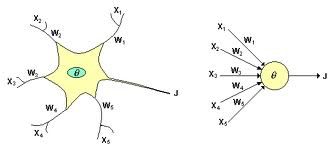
\includegraphics[width=0.7\textwidth]{figures/rna.jpg}
		\caption{Comparación de neurona artificial (derecha) y biológica (izquierda). Imagen obtenida de~\cite{rna}.}
		\label{fig.rna}
	\end{center}
\end{figure}

Tras definir el contexto general, este trabajo se centra en el Aprendizaje Profundo, situado dentro del marco de la IA, que permite obtener el conocimiento entrenando a las máquinas con ejemplos, evitando la necesidad de que los seres humanos especifiquen formalmente todo el conocimiento que necesita el ordenador. En la Figura~\ref{fig.aprendizaje}, se sitúa ésta solución en el marco de la \acrshort{ia} y sus diferentes divisiones.

\begin{figure}[H]
	\begin{center}
		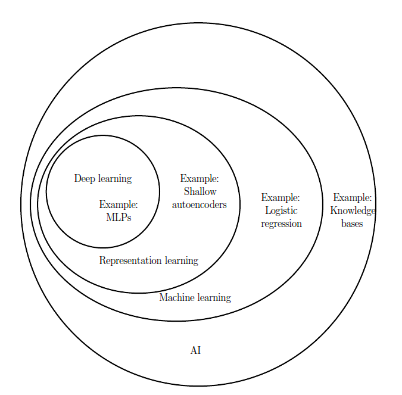
\includegraphics[width=0.6\textwidth]{figures/aprendizaje}
		\caption{Diagrama de Venn que muestra el marco de la \acrshort{ia}. Imagen obtenida de~\cite{Goodfellow-et-al-2016}.}
		\label{fig.aprendizaje}
	\end{center}
\end{figure}

En términos generales, la \acrshort{ia} contiene el Aprendizaje Máquina (\textit{Machine Learning}) definido como la capacidad de las computadoras para adquirir sus propios conocimientos, extrayendo patrones de datos sin procesar. A su vez, en el interior de la misma se sitúa el Aprendizaje de la Representación (\textit{Representation Learning}), que utiliza el aprendizaje máquina para descubrir, no sólo el mapeo de la representación a la salida, sino también la representación misma. Finalmente, en este último bloque estaría situado el Aprendizaje Profundo (\textit{Deep~Learning}), que permite a la computadora construir conceptos complejos a partir de conceptos más sencillos.\\

Dentro del aprendizaje profundo es posible aplicar diversas técnicas. La técnica más común y la que será empleada en este trabajo son las \acrfull{cnn}, que pretenden simular el funcionamiento del cerebro humano para establecer conclusiones sobre los datos introducidos a la misma. La idea básica es construir propiedades que permitan crear modelos de redes invariantes a ciertas transformaciones en las entradas.\\

Este tipo de redes tiene una estructura especial, mostrada en la Figura~\ref{fig.cnn}. Está compuesta, generalmente, por una capa convolucional, que implementa una operación de convolución, y una capa de submuestreo o agrrupación, que genera características invariantes de traducción calculando estadísticas de las activaciones de convolución a partir de un pequeño campo receptivo. Cada neurona en una capa oculta se conectará a un pequeño campo de la capa anterior, denominado campo receptivo local. En la capa convolucional, las neuronas están organizadas en múltiples capas ocultas paralelas, denominadas mapas de características, de tal manera que cada neurona en un mapa de características está conectada a un campo receptivo local. Para cada mapa de características, todas las neuronas comparten el mismo parámetro de peso que se conoce como filtro o \textit{kernel}~\cite{cnn}.

\begin{figure}[H]
	\begin{center}
		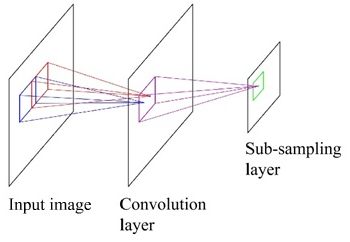
\includegraphics[width=0.4\textwidth]{figures/cnn}
		\caption{Estructura de \acrshort{cnn}. Imagen obtenida de~\cite{cnn}.}
		\label{fig.cnn}
	\end{center}
\end{figure}

En la actualidad existen múltiples disciplinas que tratan de incluir esta tecnología en su ámbito de trabajo para obtener resultados de forma más rápida y precisa. Una de las disciplinas que mas esfuerzos pone en la investigación de este campo es la medicina, cuyo principal objetivo lograr diagnosticar y tratar, e incluso prevenir enfermedades como el cáncer. Un ejemplo de ello fue llevado a cabo por el \textit{\acrfull{bidmc}} y la Escuela de Medicina de Harvard, que consiguió el premio máximo en dos categorías del \acrfull{isbi} para la detección del cáncer de mama. El equipo, utilizando la plataforma Caffe, comenzó entrenando su máquina con cientos de diapositivas marcadas para indicar qué partes tienen células cancerosas y cuáles normales, identificando qué tipo de diapositivas eran más complicadas y alimentando el sistema con muestras más difíciles. Con este método, se obtuvo un acierto 92 por ciento del tiempo y, aunque todavía no compite con los patólogos humanos,cuya precisión es el 96 por ciento del tiempo, se obtiene un gran avance en este campo~\cite{2016arXiv160605718W}.\\

\begin{figure}[H]
	\begin{center}
		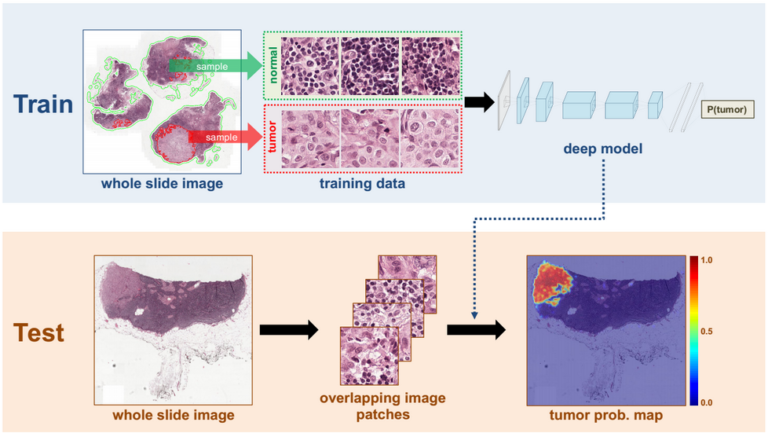
\includegraphics[width=0.6\textwidth]{figures/cancer}
		\caption{Marco utilizado para la detección del cáncer de mama. Imagen obtenida de~\cite{2016arXiv160605718W}.}
	\end{center}
\end{figure}

Un segundo ejemplo que está a la orden del día es la aplicación en la conducción autónoma. La idea de que un coche pueda manejarse en la carretera por sí mismo sin necesidad de la existencia de un conductor que realice el trabajo es tan llamativa que existen múltiples organizaciones que tratan de abarcar este problema. Existen tres paradigmas, mostrados en la Figura~\ref{fig.conduccion}, que permiten abarcar el problema de la conducción autónoma: el enfoque de percepción mediada, que analiza una escena entera para tomar una decisión de conducción, el enfoque de reflejo de comportamiento, que directamente mapea una imagen de entrada a una acción de conducción por un regresor, y el enfoque basado en la percepción directa para estimar la posibilidad para conducir. Este último fue desarrollado por la Universidad de Princeton ha desarrollado y con el se propone mapear una imagen de entrada a un pequeño número de indicadores de percepción clave que se relacionan directamente con la disponibilidad de un estado de carretera o tráfico para la conducción. Esta representación proporciona un conjunto de descripciones compactas pero completas de la escena, permitiendo a un controlador sencillo conducir de forma autónoma.

\begin{figure}[H]
	\begin{center}
		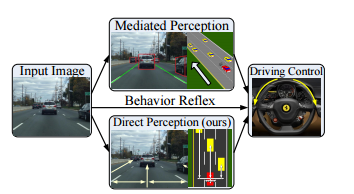
\includegraphics[width=0.6\textwidth]{figures/conduccion}
		\caption{Paradigmas de la conducción autónoma. Imagen obtenida de~\cite{2015arXiv150500256C}.}
		\label{fig.conduccion}
	\end{center}
\end{figure}

Otro ejemplo de aplicación es la traducción automática que, a pesar de haber existido durante mucho tiempo, el aprendizaje profundo consigue los mejores resultados en la traducción automática de texto e imágenes. Gracias a las \acrshort{cnn} es posible identificar las imágenes que tienen letras y donde se situan estas en la escena. Una vez identificadas, pueden convertirse en texto, traducirlo y recrear la imagen con esa traducción. Esta técnica es conocida como traducción visual instantánea~\cite{traduccion}

\begin{figure}[H]
	\begin{center}
		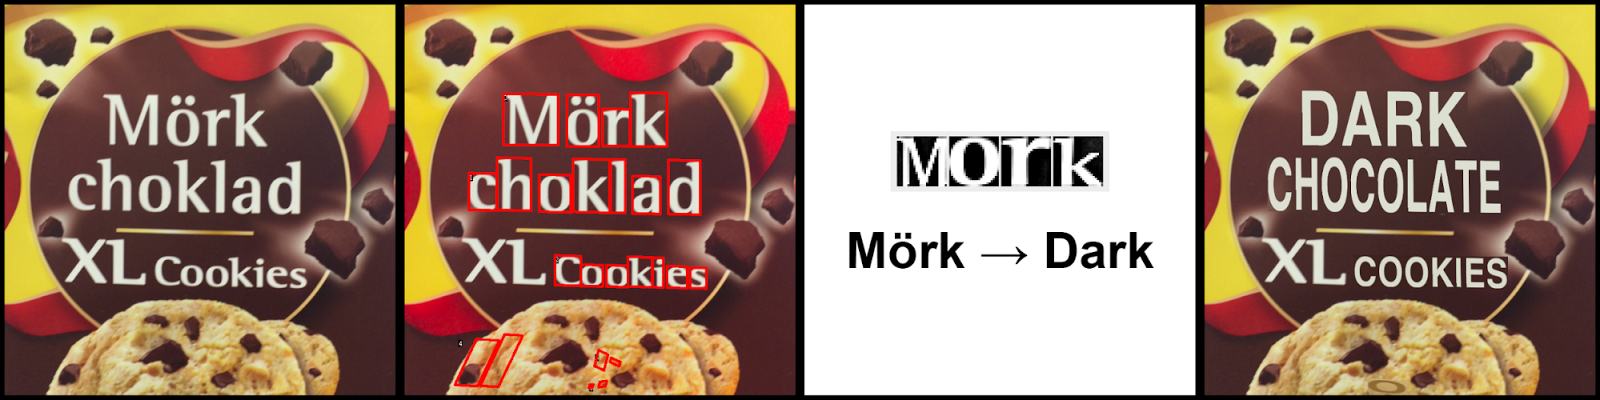
\includegraphics[width=0.6\textwidth]{figures/traduccion}
		\caption{Ejemplo de traducción visual instantánea. Imagen obtenida de~\cite{traduccion}.}
	\end{center}
\end{figure}

Un último ejemplo de aplicación de esta tecnología se basa en adición automática de sonidos a películas mudas, donde el sistema debe sintetizar sonidos para que coincidan con un video silencioso. Para esta tarea el sistema se entrena utilizando 1000 ejemplos de video con el sonido de un tambor golpeando diferentes superficies y creando diferentes sonidos. El modelo de aprendizaje profundo asocia los fotogramas de vídeo con una base de datos de sonidos pre-grabados para seleccionar un sonido que mejor se adapte a lo que está sucediendo en la escena y lo reproduzca~\cite{2015arXiv151208512O}.

\begin{figure}[H]
	\begin{center}
		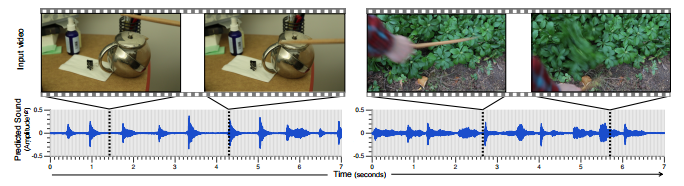
\includegraphics[width=0.8\textwidth]{figures/sonido}
		\caption{Ejemplo adición de sonidos a películas mudas. Imagen obtenida de~\cite{2015arXiv151208512O}.}
	\end{center}
\end{figure}


Además de las aplicaciones explicadas anteriormente existen muchísimas otras que surgen de las propias inquietudes del ser humano: reconocimiento facial, videovigilancia, identificación de posiciones... Sin embargo, ninguna de ellas ha sido desarrollada por completo, dejando una gran vía de investigación y desarrollo sobre el tema.\\

Este trabajo se centrará en la clasificación y detección de imágenes estáticas o en movimiento. La diferencia entre ambas aplicaciones es que la detección permite identificar en una única imagen diferentes objetos, independientemente del tamaño y la posición en la misma, según el entrenamiento que se le haya proporcionado a la misma, mientras que la clasificación identifica una imagen entrante a la red como perteneciente a una clase determinada.\\

Por último, para implementar todo lo explicado anteriormente, existen múltiples plataformas que facilitan el entrenamiento y la implementación de estas redes. TensorFlow, Keras, Theano, Caffe, Lassagne o Torch son algunos de los ejemplos más conocidos de estas plataformas. En este trabajo se utilizará la plataforma Caffe, una de las más veteranas. La elección de esta plataforma radica en el gran número de ejemplos que proporciona la misma para poder implementar en las aplicaciones sin necesidad de realizar el entrenamiento, ahorrando tiempo al desarrollador. Además está centrado en la \acrshort{va}, lugar hacia el que se enfoca este trabajo, y resulta bastante robusto y rápido.\\


\section{Objetivos}
Una vez se ha situado el trabajo en un marco definido, el objetivo general es claro: Se pretende ahondar en el mundo de la \acrshort{ia}, en concreto en técnicas de aprendizaje profundo y \acrshort{cnn}, para obtener resultados que puedan resultar interesantes y desarrollar una aplicación que permita implementar estas técnicas con la mayor exactitud posible. Este objetivo general ha sido  articulado en varios subobjetivos concretos: 

\begin{itemize}
	\item \textbf{Estudio de la plataforma Caffe.}. Se pretende entender la plataforma escogida para un correcto uso de la misma y la obtención de las redes que sean necesarias.
	\item \textbf{Desarrollo de componente que permita la clasificación de dígitos}, integrando una red entrenada con Caffe.
	\item \textbf{Estudio y mejora de redes neuronales para la clasificación de dígitos.} Se realizarán diversas pruebas para tratar de alcanzar la red más robusta posible y utilizarla en el componente desarrollado.
	\item \textbf{Primera aproximación a la detección de Caffe.} Se estudiará la detección SSD con Caffe para estímulos interesantes para aplicaciones futuras como personas, coches, bicicletas o señales de tráfico.
\end{itemize}

En la Figura~\ref{fig.diagrama} se desglosa, por semanas, el tiempo que ha llevado cada una de las tareas para la consecución de los objetivos.

\begin{figure}[H]
	\begin{center}
		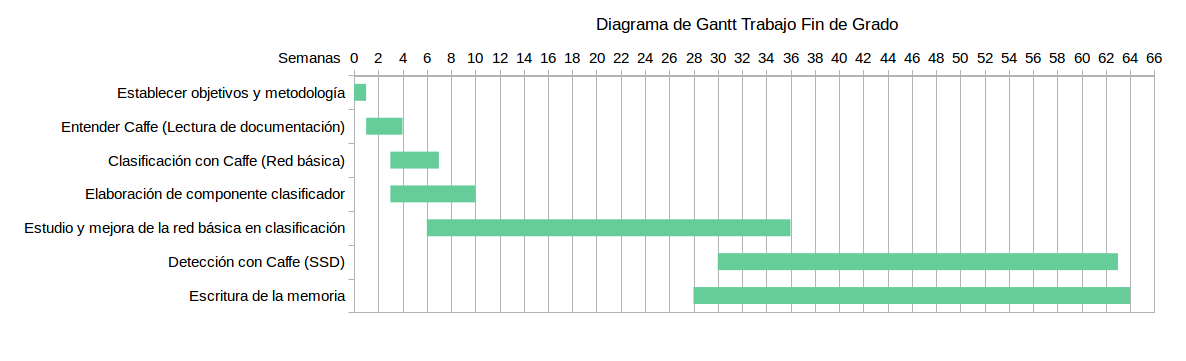
\includegraphics[width=1\textwidth]{figures/diagrama}
		\caption{Diagrama de Gantt del trabajo realizado}
		\label{fig.diagrama}
	\end{center}
\end{figure}

\section{Metodología}
Para la consecución de los objetivos marcados se han utilizado varias herramientas que han permitido el seguimiento del trabajo por todos los miembros del grupo, permitiendo a todos ellos estar al tanto del trabajo realizado y aportar los comentarios o correcciones que se consideren necesarias.\\

Como herramienta principal, se establecieron reuniones semanales con todos los miembros del grupo que permitieron poner en común y discutir los resultados obtenidos y acordar las vías a seguir durante la siguiente semana.\\

Como herramientas complementarias, se utilizaron un bitácora y un repositorio de Git Hub, que permitieron agilizar las reuniones al tener acceso de antemano al trabajo realizado. El bitácora se desarrolló empleando la \textit{Wiki} de JdeRobot~\footnote{http://jderobot.org/Noyaga-tfg}, redactando cada semana el trabajo realizado y todos los resultados obtenidos. El repositorio de Git Hub~\footnote{https://github.com/RoboticsURJC-students/2016-tfg-nuria-oyaga} permitió a todos los miembros del grupo acceder al código desarrollado, probarlo y establecer correcciones sobre el mismo.\\

El enfoque de desarrollo que se ha llevado a cabo es similiar al enfoque en espiral. Se establecen cuatro fases principales que son recorridas en forma de caracola. En primer lugar se marcaron los objetivos a alcanzar, seguido de una fase de análisis de riesgo para evaluar qué problemas era posible encontrarse al empezar el desarrollo. Tras evaluar las amenazas se procedió al propio desarrollo del trabajo y una última fase de evaluación del resultado obtenido. No existe un número fijo de iteraciones sino que se producen tantas iteraciones como sean necesarias para obtener un resultado adecuado, incrementando en cada iteración el alcance del trabajo.

\section{Estructura de la memoria}
Para mostrar el trabajo realizado y los objetivos conseguidos se elabora la memoria con la estructura mostrada a continuación.\\

En el \textbf{Capítulo 1, Introducción y objetivos,} se sitúa el trabajo en el marco actual de la tecnología, la \acrshort{ia} y la sociedad en general, para después establecer las metas que se pretenden alcanzar con el mismo.\\

El \textbf{Capítulo 2, Infraestructura,} describe todo el \textit{Software} utilizado en el proyecto, incluyendo la principal plataforma, Caffe, y los conjuntos de datos empleados para la obtención y evaluación de las redes neuronales. Además se explican los diferentes parámetros que serán empleados para evaluar las prestaciones de las redes creadas.\\

En el \textbf{Capítulo 3, Clasificación con Aprendizaje Profundo,} se expone todo el trabajo realizado para abordar el problema de la clasificación de dígitos con \acrshort{cnn}. En concreto se describe el funcionamiento de Caffe en la clasificación, el componente creado, y todas las pruebas realizadas para tratar de conseguir una red robusta, con sus correspondientes resultados.\\

En el \textbf{Capítulo 4, Detección con Aprendizaje Profundo,}  se proporciona la información necesaria para realizar la detección con Caffe y se muestran algunos resultados de pequeñas pruebas realizadas para una mejor comprensión de la misma.\\

Por útlimo, el \textbf{Capítulo 5, Conclusiones y líneas futuras,} resume todas las conclusiones obtenidas en los puntos anteriores y se establece un posible plan de actuación en un futuro para continuar la con la investigación en el tema que se aborda en el trabajo.
